\documentclass{article}
\usepackage{amsmath,amsthm,amssymb}
\usepackage{mathtext}
\usepackage[T1,T2A, T2B]{fontenc}
\usepackage[utf8]{inputenc}
\usepackage[english,russian]{babel}
\usepackage{indentfirst}

\usepackage{graphicx}
\usepackage{pgfplots}

\usepackage[14pt]{extsizes}

\usepgfplotslibrary{fillbetween}
\usetikzlibrary{patterns}

\oddsidemargin=-0.4mm
\textwidth=160mm
\topmargin=4.6mm
\textheight=210mm

\parindent=0pt
\parskip=3pt

\title{Расчетно- работа}
\date{}

\pgfplotsset{compat=1.9}
\begin{document}

\begin{titlepage}

\vspace{100pt}
\begin{center}
    \huge \textbf{Домашняя работа} \\
    \vspace{50pt}
    \huge \textbf{Графический метод решения ЗЛП}
\end{center}
\begin{flushright}

\vspace{350pt}
\begin{tabular}{rl}
     \Large Студент: & \Large Д.Д.Наумов \\
     \Large Группа: & \Large 8О-306Б-17 \\
\end{tabular}
\end{flushright}
\end{titlepage}


\subsection*{Задание}

Построить линейную оптимизационную модель и решить ЗЛП графически.

\subsection*{Условие}

Металлургический завод должен изготовить не менее 50 тонн литья, используя для этого чистую сталь и металлолом.  Отношение веса металлолома к весу чистой стали в процессе получения сплава не должно превышать 7/8. Запасы чистой стали на заводе ограничены и не превышают 40 тонн, а запасы металлолома-60 тонн.

По производственным условиям на процесс плавки и литья не может быть отведено более 18 часов, при этом на подготовку 10 тонн стали уходит 3 часа, а на 10 тонн металлолома-2 часа производственного времени.

Производственные затраты на литье в расчете на 1 тонну стали составляют 3 условных единицы, а затраты на 1 тонну металлолома-5 условных единиц.

\subsection{Решение}

Составляем систему неравенств:

$\left\{\begin{aligned}
    &0 \leq x_1 \leq 40 \\
    &0 \leq x_2 \leq 60 \\
    &x_1 + x_2 \geq 50 \\
    &\frac{x_2}{x_1} \leq \frac{7}{8} \\
    &\frac{3}{10}x_1 + \frac{2}{10}x_2 \leq 18
\end{aligned}\right. \ \ \Longrightarrow \ \
\left\{\begin{aligned}
    &0 \leq x_1 \leq 40 \\
    &0 \leq x_2 \leq 60 \\
    &x_2 \geq 50 - x_1 \\
    &x_2 \leq \frac{7}{8}x_1 \\
    &x_2 \leq90 -\frac{3}{2}x_1
\end{aligned}\right.$

\vspace{10pt}

$f(x) = 3x_1 + 5x_2 \rightarrow \min$ или $x_2 = -\frac{3}{5}x_1 + a$, где $a \rightarrow \min$

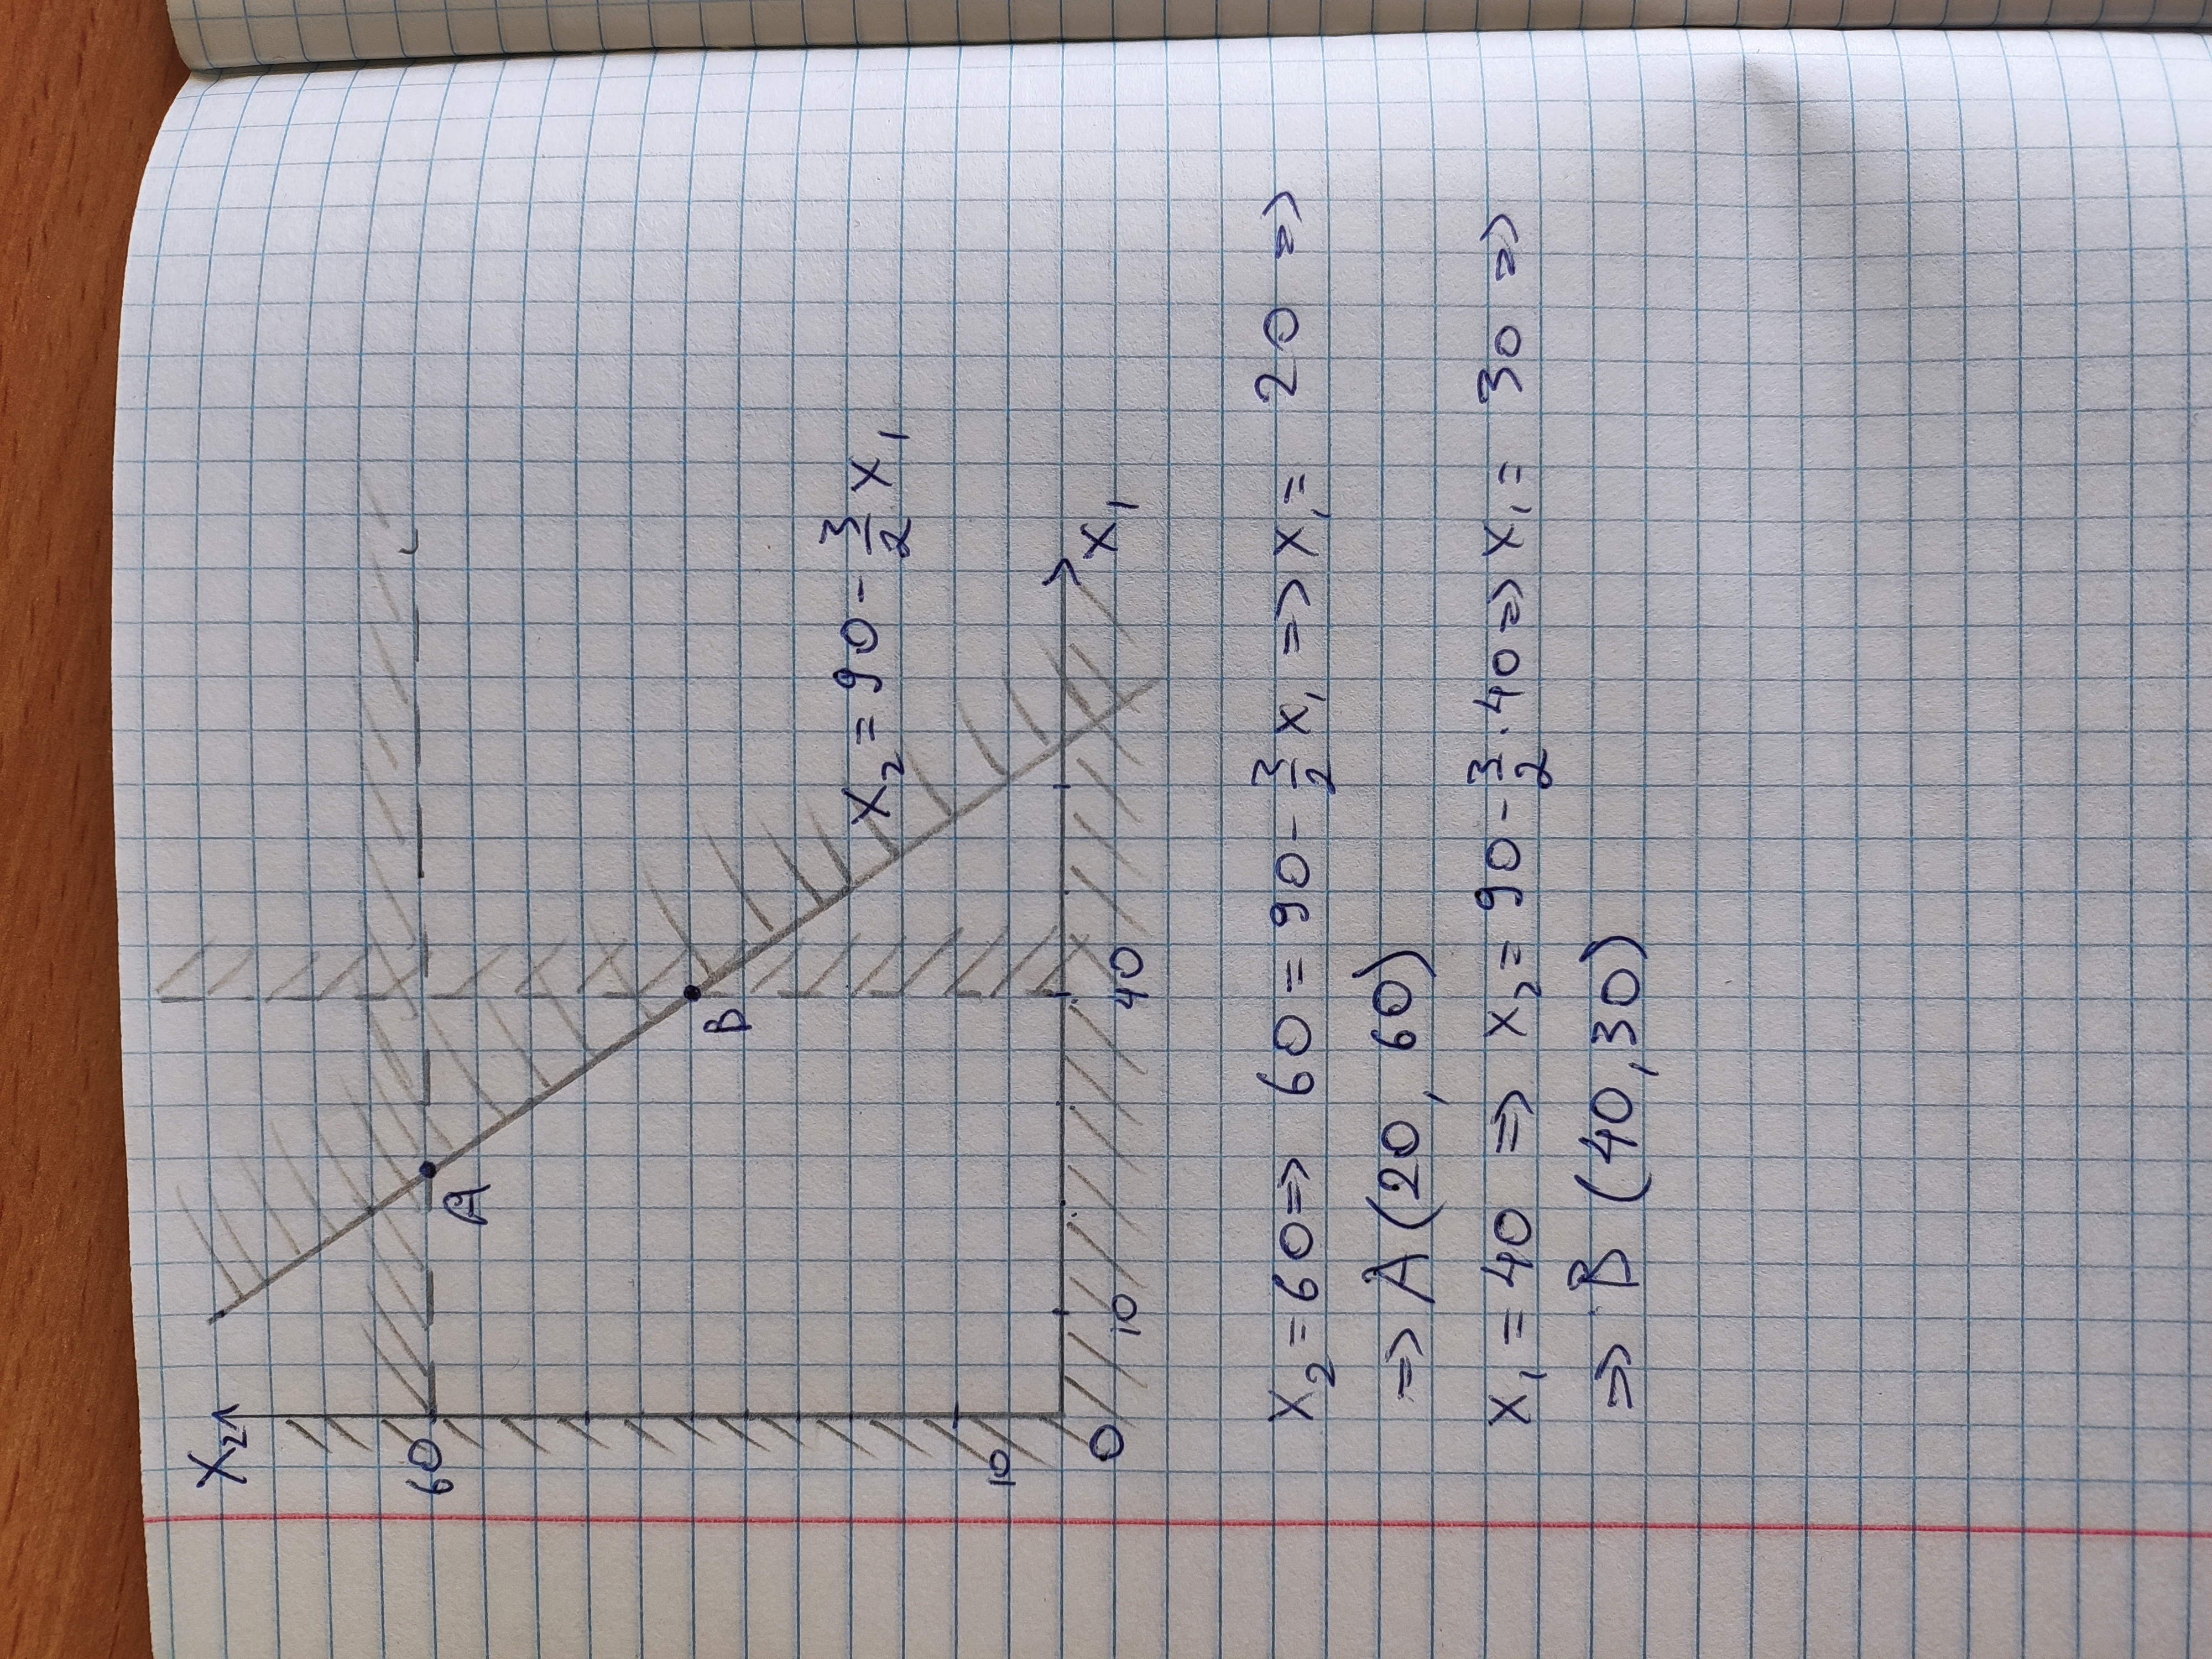
\includegraphics[angle=-90, width=0.8\linewidth]{1.jpg}\\

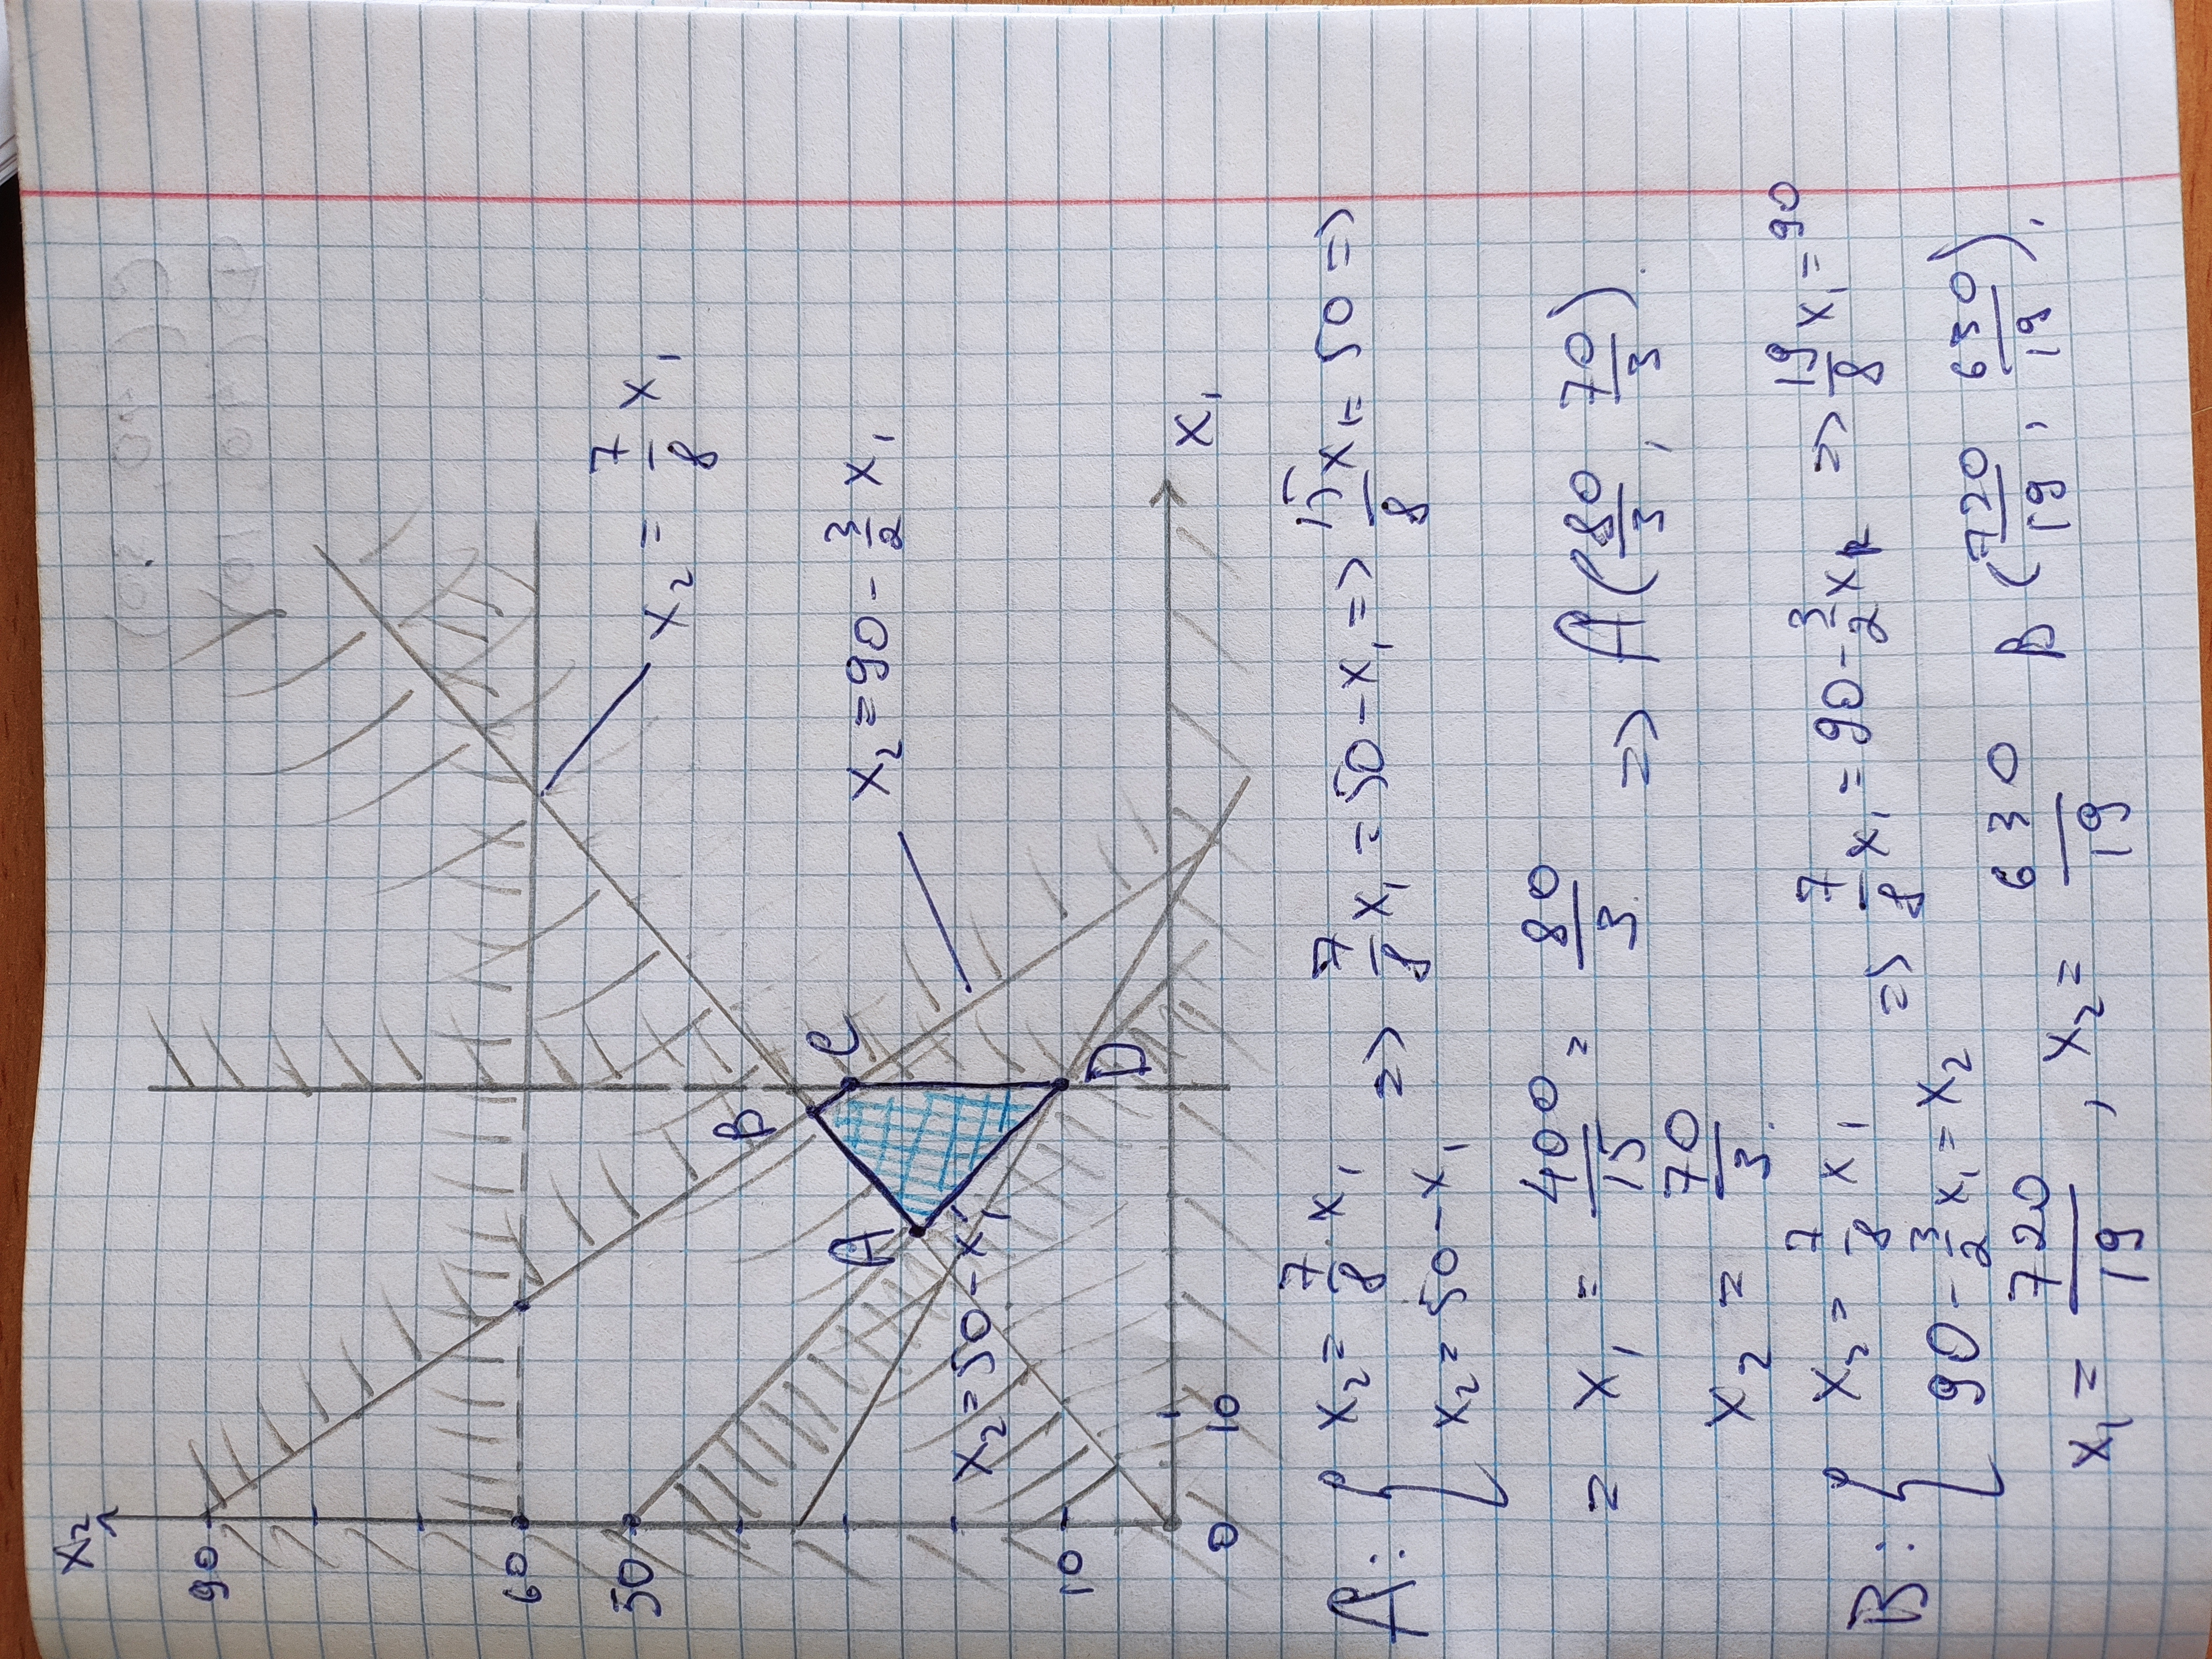
\includegraphics[angle=-90, width=0.8\linewidth]{2.jpg}\\

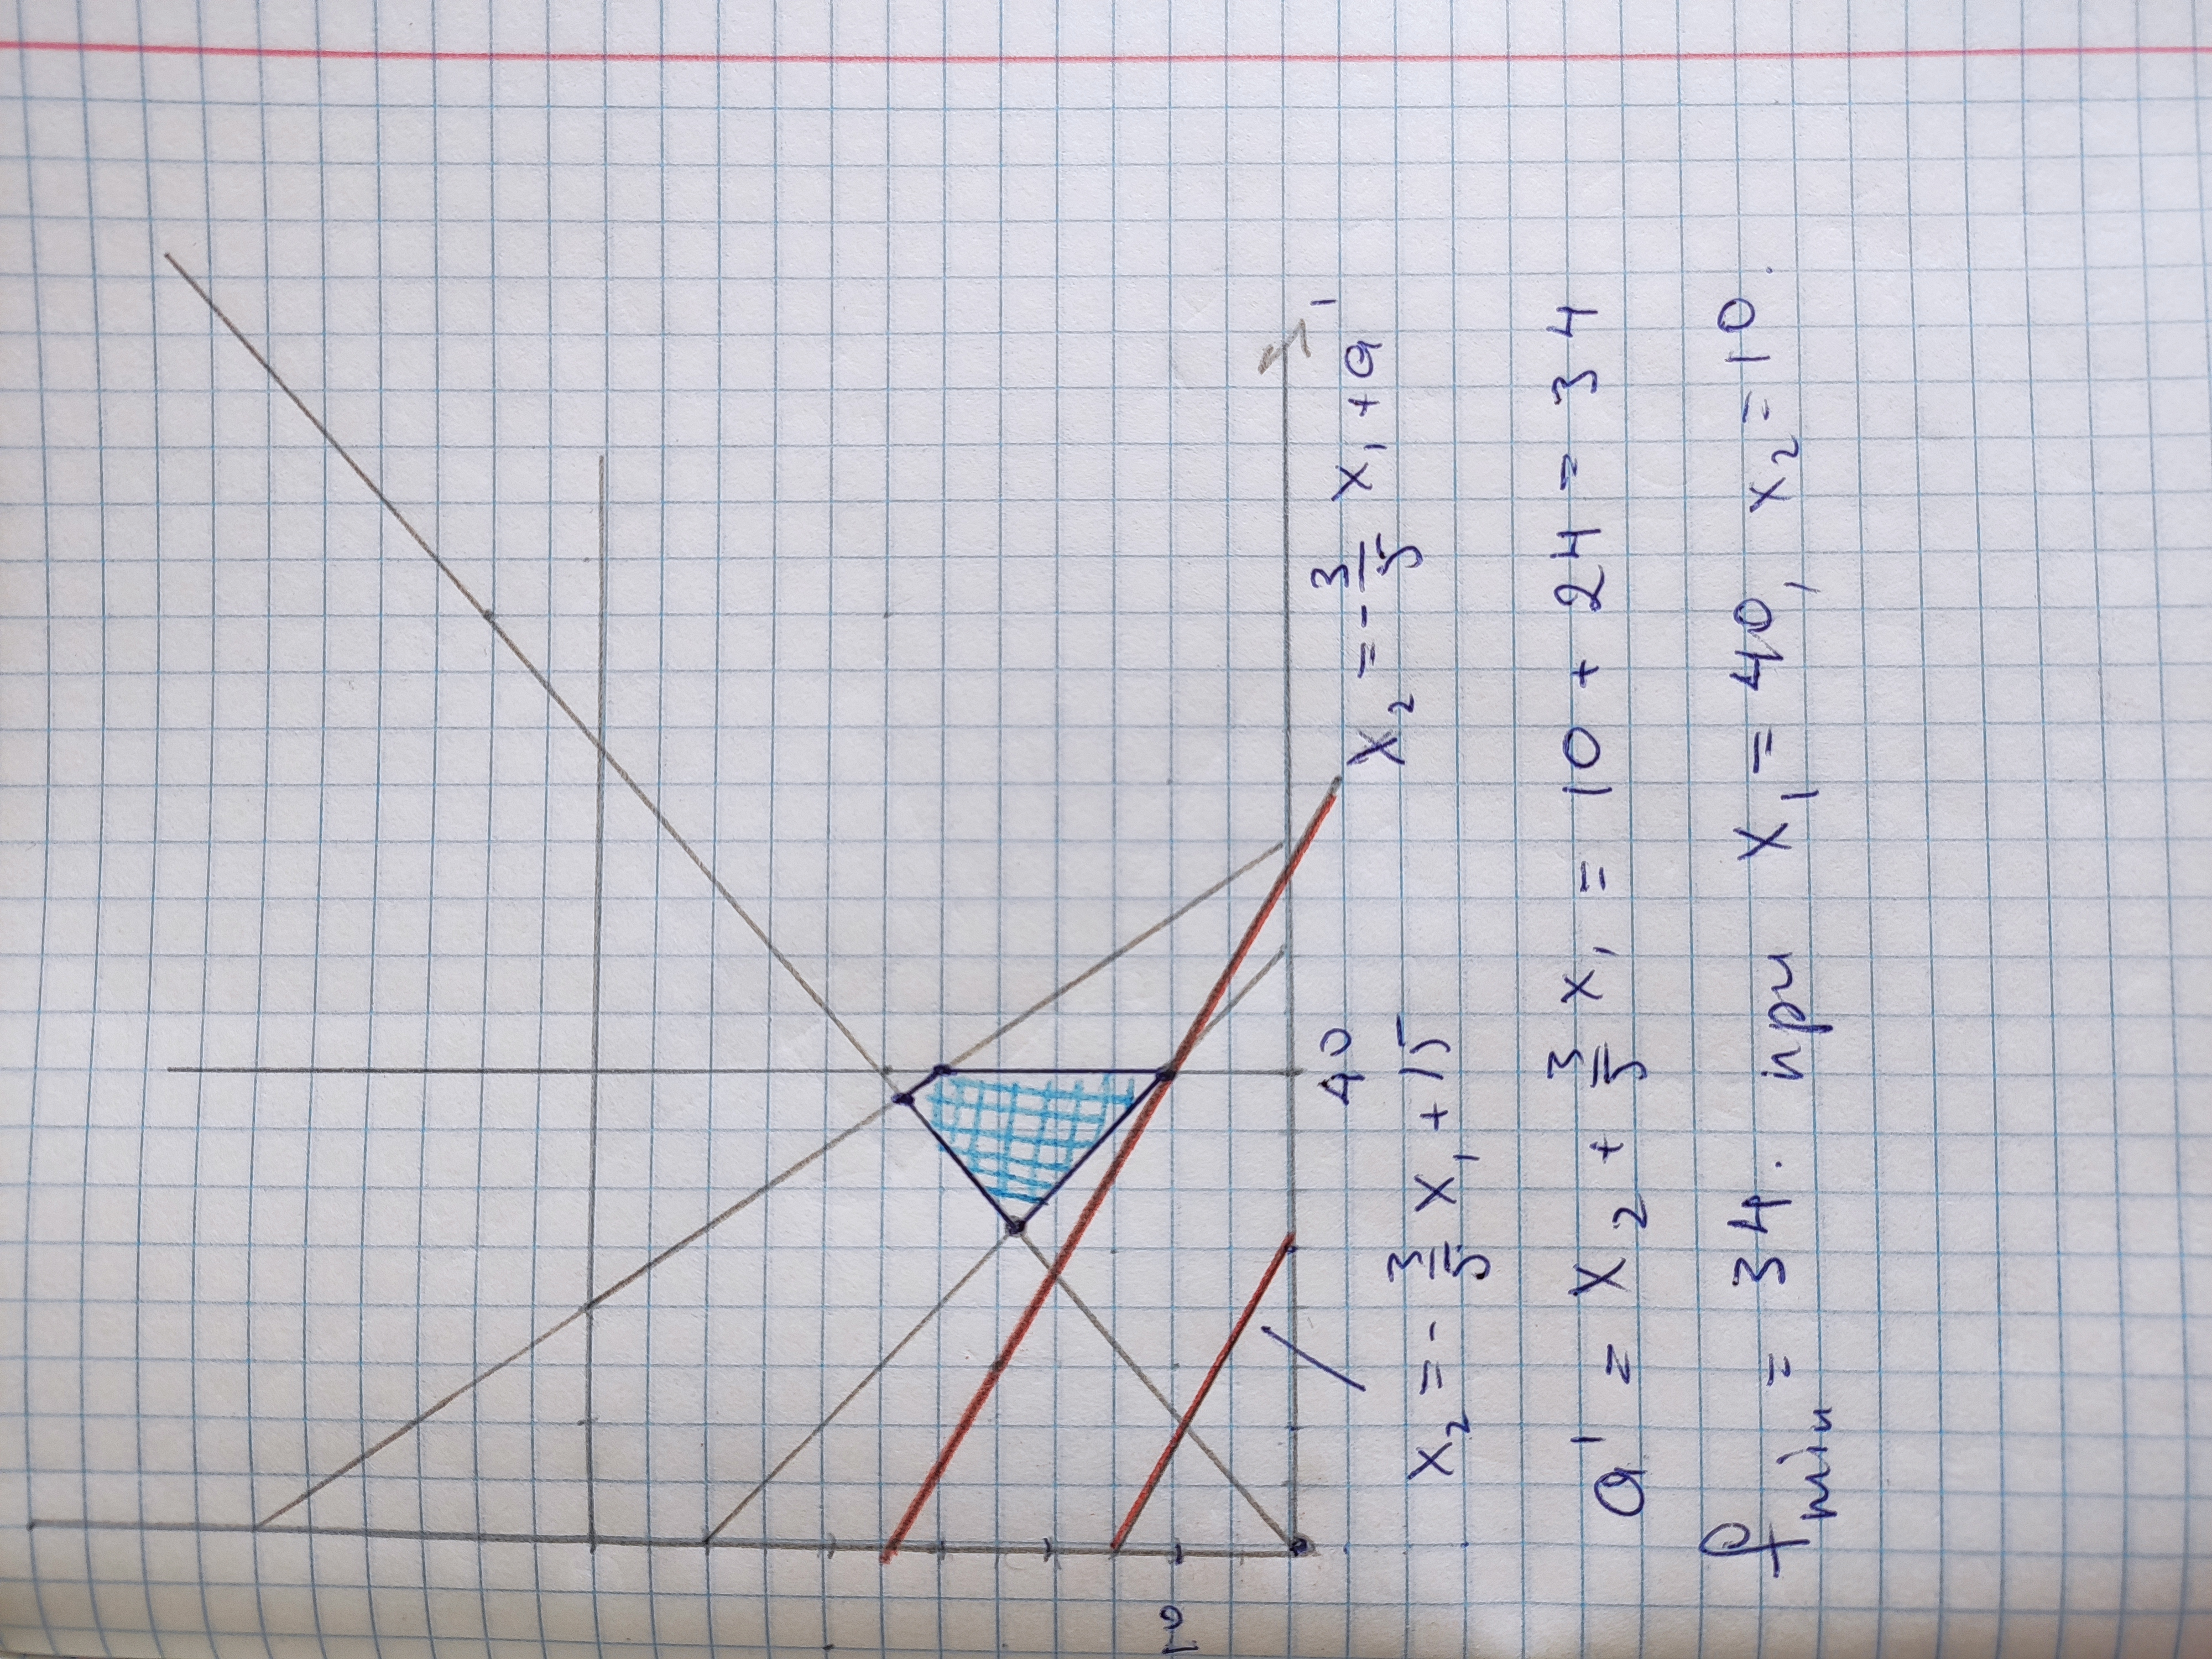
\includegraphics[angle=-90, width=0.8\linewidth]{3.jpg}\\

\end{document}
